% file: DNN.tex
%
% github        : ernestyalumni
% gmail         : ernestyalumni 
% linkedin      : ernestyalumni 
% wordpress.com : ernestyalumni
%
% This code is open-source, governed by the Creative Common license.  Use of this code is governed by the Caltech Honor Code: ``No member of the Caltech community shall take unfair advantage of any other member of the Caltech community.'' 

\documentclass[10pt]{amsart}
\pdfoutput=1
\usepackage{mathtools,amssymb,lipsum,caption}

\usepackage{graphicx}
\usepackage{hyperref}
\usepackage[utf8]{inputenc}
\usepackage{listings}
\usepackage[table]{xcolor}
\usepackage{pdfpages}
\usepackage{tikz}
\usetikzlibrary{matrix,arrows,backgrounds}

\usepackage{breqn} % for dmath


\usepackage{cancel} % for Feynman slash notation

\hypersetup{colorlinks=true,citecolor=[rgb]{0,0.4,0}}


%\oddsidemargin=15pt
%\evensidemargin=5pt
%\hoffset-45pt
%\voffset-55pt
%\topmargin=-4pt
%\headsep=5pt
%\textwidth=1120pt
%\textheight=595pt
%\paperwidth=1200pt
%\paperheight=700pt
%\footskip=40pt








\newtheorem{theorem}{Theorem}
\newtheorem{corollary}{Corollary}
%\newtheorem*{main}{Main Theorem}
\newtheorem{lemma}{Lemma}
\newtheorem{proposition}{Proposition}

\newtheorem{definition}{Definition}
\newtheorem{remark}{Remark}

\newenvironment{claim}[1]{\par\noindent\underline{Claim:}\space#1}{}
\newenvironment{claimproof}[1]{\par\noindent\underline{Proof:}\space#1}{\hfill $\blacksquare$}

%This defines a new command \questionhead which takes one argument and
%prints out Question #. with some space.
\newcommand{\questionhead}[1]
  {\bigskip\bigskip
   \noindent{\small\bf Question #1.}
   \bigskip}

\newcommand{\problemhead}[1]
  {
   \noindent{\small\bf Problem #1.}
   }

\newcommand{\exercisehead}[1]
  { \smallskip
   \noindent{\small\bf Exercise #1.}
  }

\newcommand{\solutionhead}[1]
  {
   \noindent{\small\bf Solution #1.}
   }


  \title[Deep Neural Networks from a practical Category Theory point of view)]{Deep Neural Networks from a practical Category Theory point of view}

\author{Ernest Yeung \href{mailto:ernestyalumni@gmail.com}{ernestyalumni@gmail.com}}
\date{14 juiellet 2017}
\keywords{Machine Learning, Neural Networks, Deep Neural Networks, Category Theory, R-Modules, CUDA C/C++, theano, tensorflow}

\begin{document}

\definecolor{darkgreen}{rgb}{0,0.4,0}
\lstset{language=Python,
 frame=bottomline,
 basicstyle=\scriptsize,
 identifierstyle=\color{blue},
 keywordstyle=\bfseries,
 commentstyle=\color{darkgreen},
 stringstyle=\color{red},
 }
%\lstlistoflistings

\maketitle

\tableofcontents

%\begin{multicols*}{2}


 











\begin{abstract}
\section{Summary}
I make the case to view Deep Neural Networks (DNN) from a practical Category Point of view, namely to consider the algebraic properties of tensors and $R$-modules and how the elements of a DNN are represented by such mathematical objects.  I do this to place the mathematical formulation of DNNs as general (and rigorous) as possible.  I also do this, for practical reasons, to provide a concrete software design pattern, in object-oriented programming (OOP), in implementing DNNs.  There should be a 1-to-1 correspondence, isomorphism, between a DNN's mathematical description and OOP design pattern, so to have a universally agreed upon OOP hierarchy.  

Finally, I provide a working implementation of DNNs in Python, in both \verb|theano| and \verb|tensorflow| frameworks.  
\end{abstract}

%Also, I would argue that it makes the deployment of various DNNs easier (to specify).  

% on how classes, functions, variables, etc. should be implemented

For an introduction to Neural Networks (NN) or i.e. Deep Neural Networks, I will reference the Coursera "MOOC" (Massive Open Online Course) by Prof. Andrew Ng, "Machine Learning Introduction."\cite{AnNg}

First, I will expound upon the rationale for representing input data as right $R$-modules.  

\section{Input Data as Right $R$-modules}

Consider, as a start, the total given (training) input data, consisting of $m\in \mathbb{Z}^+$ (training) examples, each example, say the $i$th example, being represented by a "feature" vector of $d$ features, $X^{(i)} \in \mathbb{K}^d$, where $\mathbb{K}$ is a field or (categorical) classes, i.e. as examples of fields, the real numbers $\mathbb{R}$, or integers $\mathbb{Z}$, so that $\mathbb{K} = \mathbb{R},\mathbb{Z}$ or $\mathbb{K} = \lbrace 0 ,1,\dots K-1\rbrace$, where $K$ is the total number of classes that a feature could fall into (for "categorical data").  Note that for this case, the case of $\mathbb{K}=\lbrace 0 ,1,\dots K-1\rbrace$, for $K$ classes, though labeled by integers, this set of integer labels is \emph{not} equipped with ordered field properties (it is meaningless to say $0<1$, for example), nor the usual field (arithmetic) operations (you cannot add, subtract, multiply, or even take the modulus of these integers).  

How can we "feed into" our machine such (categorical) class data?  Possibly, we should intuitively think of the Kronecker Delta function:
\[
\delta_{iJ} = \begin{cases} 0 & \text{ if } i\neq J \\ 
 1 & \text{ if } i = J \end{cases}
\]
for some (specific) class $J$, represented by an integer.  So perhaps our machine can learn kronecker delta, or "signal"-like functions that will be "activated" if the integer value of a piece (feature) of data is exactly equal to $J$ and $0$ otherwise.  This is essentially what the so-called "one-hot encoding" does in turning "categorical data" (some finite set) into a numerical value (a vector of $0$s and $1$s of dimension that is equal to the number of classes).  

Onward, supposing $\mathbb{K}$ is a field, consider the total given input data of $m$ examples:
\[
\lbrace X^{(i)} \in \mathbb{K}^d\rbrace^m_{i=1,2,\dots m}
\]
One can arrange such input data into a $m\times d$ matrix.  We want to do this, for one reason, to \emph{take advantage of the parallelism afforded by GPU(s)}.  Thus we'd want to act upon the entire input data set $\lbrace X^{(i)} \in \mathbb{K}^d\rbrace^m_{i=1,2,\dots m}$.  

We'd also want to, in the specific case of using the \verb|theano| framework, do \emph{parallel reduce} in order to do a \emph{summation}, $\sum_{i=1}^m$, over all (training) examples, to obtain a cost function(al) $J$ \cite{theano}.  

For \verb|theano|, parallel \verb|reduce| and \verb|scan| operations can only be done over the first (size) dimension of a \verb|theano| tensor\cite{theano}.  Thus, we write the total input data as such:
\begin{equation}
\lbrace X^{(i)} \in \mathbb{K}^d\rbrace^m_{i=1,2,\dots m} \mapsto X^{(i)}_j \in \text{Mat}_{\mathbb{K}}(m,d)
\end{equation}
i.e. $X^{(i)}_j$ is a $m\times d$ matrix of $\mathbb{K}$ values, with each $i$th row corresponding to the $i=1,2,\dots m$th example,  and $j$th column corresponding to the $j=1,2,\dots d$th feature (of the feature vector $X^{(i)} \in \mathbb{K}^d$).  

Let's, further make the following abstraction in that the input data $\lbrace X^{(i)} \in \mathbb{K}^d\rbrace^m_{i=1,2,\dots m}$ is really an element of a right $R$-module $\mathbf{X}$, in the category of right $R$-modules $\text{\textbf{Mod}}_R$ with ring $R$, $R$ not necessarily being commutative (see Rotman (2010) \cite{JRotman2010} for an introduction on non-commutative $R$-modules).    

A reason for this abstraction is that if we allow the underlying ring $R$ to be a field $\mathbb{K}$, (e.g. $\mathbb{K}=\mathbb{R},\mathbb{Z}$), then the "usual" scalar multiplication by scalars is recovered.  But we also need to equip $X\in \text{\textbf{Mod}}_R$ with a \emph{right action}, where ring $R$ is \emph{noncommutative}, namely 
\[
R = \text{Mat}_{\mathbb{K}}(d,s) \cong L(\mathbb{K}^d, \mathbb{K}^s)
\]
where $\text{Mat}_{\mathbb{K}}(d,s)$ denotes the ring of all matrices over field $\mathbb{K}$ of matrix (size) dimensions $d\times s$ (it has $d$ rows and $s$ columns), $\cong$ is an isomorphism, $L(\mathbb{K}^d,\mathbb{K}^s)$ is the space of all (linear) maps from $\mathbb{K}^d$ to $\mathbb{K}^s$.  If $\mathbb{K}$ is a field, this isomorphism exists.  

Thus, for 
\begin{equation}
\begin{aligned}
	& X\in \mathbf{X} \in \text{Mod}_R \\
	&  R = \text{Mat}_{\mathbb{K}}(d,s) \cong L(\mathbb{K}^d,\mathbb{K}^s)
\end{aligned}
\end{equation}

\section{Introducing $\Theta$, representing the "weights" of a DNN, as a mapping (homomorphism) between $R$-modules}

Let $\Theta \in R$. $\Theta$ is also known as the "parameters" or "weights" (and is denoted by $w$ or $W$ by others).  

Consider, as a first (pedagogical) step, only a single example ($m=1$).  $X$ is only a single feature vector, $X\in \mathbb{K}^d$.  Then for basis $\lbrace e_{\mu} \rbrace_{\mu=1\dots d}$ of $\mathbb{K}^d$, corresponding dual basis $\lbrace e^{\mu} \rbrace_{\mu=1\dots d}$ (which is a basis for dual space $(\mathbb{K}^d)^*$), then
\[
\begin{gathered}
	X\Theta = X^{\mu} e_{\mu} ( \Theta^{\ \   j}_{  \nu} e^{\nu}  \otimes e_j ) =  \qquad \quad \, \\
X^{\mu} \Theta^{\ \  j}_{  \nu}  e^{\nu}(e_{\mu})  \otimes e_j   = X^{\mu} \Theta^{\ \   j}_{  \nu}  \delta^{\nu}_{\mu} = \\  e_j = X^{\mu} \Theta^{\ \   j}_{ \mu} e_j  \text{ where } \\
\begin{aligned} & \mu , \nu = 1 \dots d \\ 
&  j = 1\dots s \end{aligned} 
\end{gathered}
\]
In this case where $X$ is simply a vector, one could think of $X$ as a "row matrix" and $\Theta$ is a matrix, acting on the right, in matrix multiplication.    

One should note that while it is deceptively simple to consider tensors as the Cartesian product, $(\mathbb{K}^d)^* \times \mathbb{K}^s$, i.e. that in general, 
\[
(\mathbb{K}^d)^* \times \mathbb{K}^s \neq T^{(d,s)}
\]
where $T^{(d,s)}$ is the set of all tensors of rank $(d,s)$ (depending upon so-called covariant, contravariant convention).  Rather, one should take the quotient of this "raw" Cartesian product with the equivalence relation of a particular submodule (which essentially defines what the zero equivalence class is; cf. Jeffrey Lee (2009) \cite{JLee2009}, Conlon (2008) \cite{Conl2008}).  It would be interesting to verify this point in terms of the needs for a tensor representation of the "weights" of a DNN.  

Now suppose, in general, $X \in \textbf{X} \in \text{\textbf{Mod}}_R$, where $X$ could be a $m\times d$ matrix, or higher-dimensional tensor.  For a concrete example, say $\textbf{X} = \text{Mat}_{\mathbb{K}}(m,d)$.  We not only have to equip this right $R$-module with the usual scalar multiplication, setting ring $R=\mathbb{K}$, but also the right action version of matrix multiplication, so that $R = \text{Mat}_{\mathbb{K}}(d,s)$.  This $R$ is \emph{non-commutative}, thus, necessitating the abstraction to right $R$-modules.  

Also, from a practical point of view, we'd like our model to take an arbitrary number of samples/examples, $m \in \mathbb{Z}^+$.  To encode this, for example in \verb|tensorflow|, this is done by setting the so-called \verb|shape| parameter to have a value of \verb|None| - the shape will be finally specified when a \verb|tf.Session| is instantiated and the computational graph is run with class method \verb|.run|.  But the mapping or computation must proceed without knowing exactly the value of $m$, and so the weights and bias $(\Theta,b)$ act \emph{on the right}.  

Indeed, for
\[
\begin{gathered}
	\Theta \in L( \text{Mat}_{\mathbb{K}}(m,d), \text{Mat}_{\mathbb{K}}(m,s) ) \cong    (\text{Mat}_{\mathbb{K}}(m,d))^* \otimes \text{Mat}_{\mathbb{K}}(m,s) \cong \text{Mat}_{\mathbb{K}}(d,s), \text{ and so } \\
%	\Theta \cong w\otimes \alpha, \quad \, w \in   \text{Mat}_{\mathbb{K}}(m,s), \, \alpha \in (\text{Mat}_{\mathbb{K}}(m,d))^*, \text{ then } \\ 
%X\Theta = X w\otimes \alpha = w \otimes \alpha(X) = w \alpha(X) \in \text{Mat}_{\mathbb{K}}(m,s)
X\Theta \in \text{Mat}_{\mathbb{K}}(m,s)
\end{gathered}
\]
%with 
%\[
%\begin{gathered}
%	\alpha(X) \in \text{Mat}_{\mathbb{K}}(d,s)  \\ 
%\end{gathered}
%\]
Further
\[
X\Theta \in \text{Mat}_{\mathbb{K}}(m,s) \in \text{\textbf{Mod}}_R
\]
with ring $R$ in this case being $R=\text{Mat}_{\mathbb{K}}(s,s_2) \cong L(\mathbb{K}^s, \mathbb{K}^{s_2})$.  

Since $X\Theta$ is an element in a $R$-module, it is an element in an (additive) abelian group.  We can add the "intercept vector" $b$ (in theano, it'd be the usual theano vector, but with its dimensions "broadcasted" for all $m$ examples, i.e. for all $m$ rows).  
\[
X\Theta + b \in \text{Mat}_{\mathbb{K}}(m,s)
\]
Considering these 2 operations on $X$, the "matrix multiplication on the right" or right action $\Theta$, and addition by $b$ together, through \emph{composition}, $(\Theta,b)$, we essentially have
\begin{equation}
\boxed{ X\in \mathbf{X} \in \text{\textbf{Mod}}_{R_1} \xrightarrow{ (\Theta,b) } X\Theta + b \in \mathbf{X_2} \in \text{\textbf{Mod}}_{R_2}  }
\end{equation}
where
\[
\begin{aligned}
& R_1 = \text{Mat}_{\mathbb{K}}(d,s_1) \cong L(\mathbb{K}^d, \mathbb{K}^{s_1} ) \\ 
& R_2 = \text{Mat}_{\mathbb{K}}(s_1,s_2) \cong L(\mathbb{K}^{s_1}, \mathbb{K}^{s_2})
\end{aligned}
\]

%\section{Axons and Deep Neural Networks (DNN)} \label{Sec:DNN}

\section{Axons: what matters is not the specific nature of objects alone, but the relationships between objects} \label{Sec:Axons}

Consider a(n artificial) neural network (NN) of $L+1 \in \mathbb{Z}^+$ "layers" representing $L+1$ neurons, with each layer or neuron represented by a vector $a^{(l)} \in \mathbb{K}^{s_l}$, $s_l \in \mathbb{Z}^+$, $l=1,2,\dots L+1$ (or, counting from $0$, $l=0,1,\dots L$, so-called $0$-based counting).  Again, $\mathbb{K}$ is either a field (e.g. $\mathbb{K}=\mathbb{R},\mathbb{Z}$), or categorical classes (which is a subset of $\mathbb{Z}^+$, but without any field properties, or field operations).  

%Nevertheless, for this pedagogical example, currently, let $\mathbb{K}=\mathbb{R}$.  

Recall the usual (familar) NN, accepting that we do right action multiplications (matrices act on the right, vectors are represented by "row vectors", which, actually, correspond 1-to-1 with \verb|numpy|/\verb|theano|/\verb|tensorflow| arrays, exactly, in that 1-dimensional arrays in \verb|numpy|/\verb|theano|/\verb|tensorflow| default to being treated as row vectors).  

Recall also that the sigmoidal or (general) \emph{activation} function, $\psi^{(l)}$, acts element-wise on a vector, matrix, or tensor.  And so 
\[
\begin{aligned}
	& \psi^{(l)}:\mathbb{K}^d \to \mathbb{K}^d \\ 
	& \psi^{(l)}: a^{(l)}_i \mapsto \psi^{(l)}(a_i^{(l)}) \qquad \, \forall \, i =0,1, \dots d-1  \\
	& \psi^{(l)} : \text{Mat}_{\mathbb{K}}(d,s) \to \text{Mat}_{\mathbb{K}}(d,s) \\
	& \psi^{(l)} : X^{(l)}_{ij} \to \psi^{(l)}(X^{(l)}_{ij} )  
\end{aligned}
\]
To generalize this, $\psi^{(l)}$ maps an $R$-module in $\text{Mod}_R$ to another $R$-module, but belonging in the same domain:
\[
\psi^{(l)} :\text{Mod}_R \to \text{Mod}_R
\]
and its operation on each "entry" of a $R$-module is clear.  

The $l$th layer was computed from the "last" or "previous" layer, in a sequence of layers, as computed as follows: 
\begin{equation}
\begin{aligned}
	& z^{(l)} := a^{(l-1)} \Theta^{(l)} + b^{(l)} \\
	& a^{(l)} := \psi^{(l)}(z^{(l)})
\end{aligned}
\end{equation}
where $\Theta^{(l)},b^{(l)}$ is as above, except there will be a total of $L$ of these tuples ($l=1,2,...L$).  

%An "axon" between 2 layers, such as layer $l$ and layer $l+1$, is mathematically computed as follows:

With $(\Theta^{(l)}, b^{(l)})$ representing the (right action) linear transformation 
\begin{equation}
%\boxed{ 
(\Theta^{(l)}, b^{(l)}) (a^{(l-1)}) := a^{(l)} \Theta^{(l)} + b^{(l)} 
%}
\end{equation}
essentially,
\begin{equation}
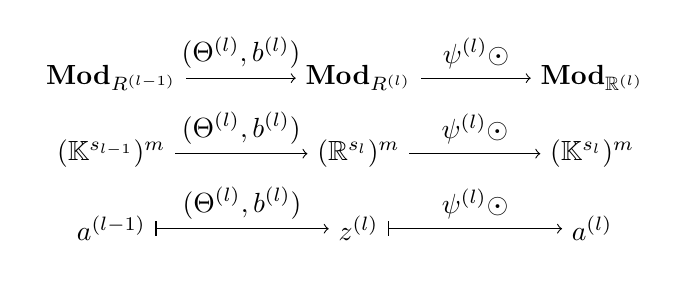
\begin{tikzpicture}
  \matrix (m) [matrix of math nodes, row sep=1.1em, column sep=4em, minimum width=1em]
  {
\text{\textbf{Mod}}_{R^{(l-1)}} & \text{\textbf{Mod}}_{R^{(l)}} & \text{\textbf{Mod}}_{\mathbb{R}^{(l)}} \\ 
(\mathbb{K}^{s_{l-1}})^m & (\mathbb{R}^{s_{l}})^m & (\mathbb{K}^{s_{l}})^m  \\ 
a^{(l-1)} & z^{(l)} & a^{(l)} \\ 
};
  \path[->]
  (m-1-1) edge node [above] {$(\Theta^{(l)}, b^{(l)})$} (m-1-2)
  (m-1-2) edge node [above] {$\psi^{(l)} \odot$ } (m-1-3)
  ;
\path[->]
  (m-2-1) edge node [above] {$(\Theta^{(l)}, b^{(l)})$} (m-2-2)
  (m-2-2) edge node [above] {$\psi^{(l)} \odot$ } (m-2-3)
  ;
\path[|->]
  (m-3-1) edge node [above] {$(\Theta^{(l)}, b^{(l)})$} (m-3-2)
  (m-3-2) edge node [above] {$\psi^{(l)} \odot$ } (m-3-3)
  ;
\end{tikzpicture}
\end{equation}

Since we need to operate with the activation function $\psi^{(l)} \odot$ elementwise, we (implicitly) equip $\text{\textbf{Mod}}_{R^{(l+1)}}$ with the Hadamard product.  In fact, with composition, we can represent the above mapping between the $l-1$ and $l$th layers as 
\begin{equation}\label{Eq:Axon}
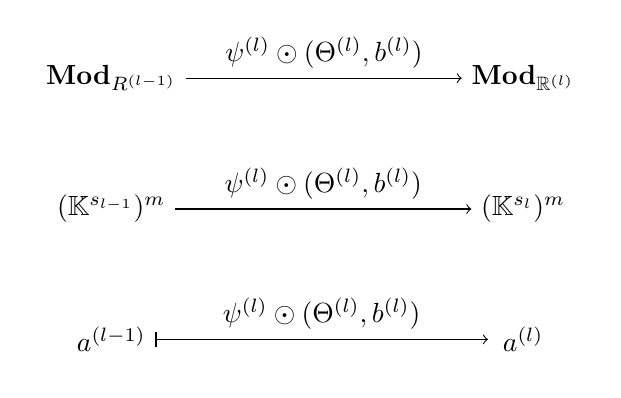
\begin{tikzpicture}
  \matrix (m) [matrix of math nodes, row sep=3.1em, column sep=10em, minimum width=2.5em]
  {
\text{\textbf{Mod}}_{R^{(l-1)}}   & \text{\textbf{Mod}}_{\mathbb{R}^{(l)}} \\ 
(\mathbb{K}^{s_{l-1}})^m  & (\mathbb{K}^{s_{l}})^m  \\ 
a^{(l-1)}  & a^{(l)} \\ 
};
  \path[->]
  (m-1-1) edge node [above] {$\psi^{(l)} \odot (\Theta^{(l)}, b^{(l)})$} (m-1-2)
  ;
\path[->]
  (m-2-1) edge node [above] {$\psi^{(l)} \odot (\Theta^{(l)}, b^{(l)})$} (m-2-2)
  ;
\path[|->]
  (m-3-1) edge node [above] {$\psi^{(l)} \odot (\Theta^{(l)}, b^{(l)})$} (m-3-2)
  ;
\end{tikzpicture} 
\end{equation}
The lesson (and the whole point of category theory) is this: instead of thinking of layers, each separately, think of or focus on the relationship, the relations, between each layers, as one whole entity.  Indeed, the historical development, and its defining characteristic, of category theory is that what does not matter is the specific nature of the mathematical objects by themselves, but the general relationship between the mathematical objects.  Thus, I propose considering the whole of the mapping shown in Eq. \ref{Eq:Axon} an \textbf{axon}.  The $l$th axon, for $l=1,2,\dots L$, is a map between the $(l-1)$th layer and the $l$th layer.  There are $L$ total axons in a NN, with $L+1$ layers (which include an input and output layer).    

To reiterate, the axon consists of the map $\psi^{(l)} \odot (\Theta^{(l)},b^{(l)})$, and the spaces it maps between, $\text{\textbf{Mod}}_{R^{(l-1)}}$ to $\text{\textbf{Mod}}_{R^{(l)}}$.  

\section{Deep Neural Networks (DNN) from the Category Point of View} \label{Sec:DNN}


Suppose we "feed in" input data $X$ into the first or $0$th layer of this NN.  This means that for $a^{(0)} \in \mathbb{R}^d$, 
\[
a^{(0)} = X^{(i)}
\]
for the $i$th (training) example.  

The "output" layer, layer $L$, should output the \emph{predicted} value, given $X$.  So 
\[
a^{(L)} \in \mathbb{R} \text{ or } \lbrace 0 ,1 , \dots K-1\rbrace \text{ or } [0,1]
\]
for regression, or classification (so it takes on discrete values) or the probability likelihood of being in some class $k$, respectively. 
 
The entire DNN can mathematically expressed as follows: 
\begin{equation}\label{Eq:DNNdiagram}
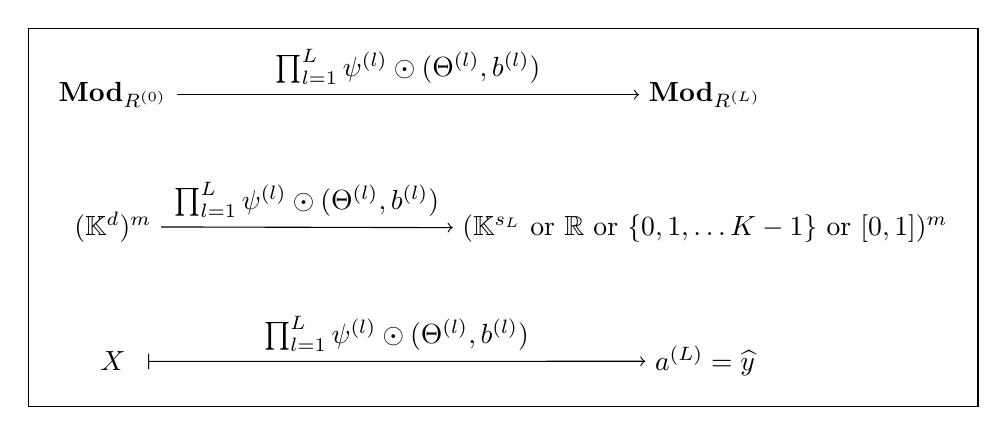
\begin{tikzpicture}[framed]
  \matrix (m) [matrix of math nodes, row sep=3.1em, column sep=10em, minimum width=2.5em]
  {
	\text{\textbf{Mod}}_{R^{(0)}} & \text{\textbf{Mod}}_{R^{(L)}}  \\
(\mathbb{K}^{d})^m  & (\mathbb{K}^{s_L} \text{ or } \mathbb{R} \text{ or } \lbrace 0 ,1,\dots K-1\rbrace \text{ or } [0,1])^m  \\ 
X  & a^{(L)}  =\widehat{y} \\ 
};
  \path[->]
  (m-1-1) edge node [above] {$\prod_{l=1}^{L} \psi^{(l)} \odot (\Theta^{(l)}, b^{(l)})$} (m-1-2)
  ;
\path[->]
  (m-2-1) edge node [above] {$\prod_{l=1}^{L} \psi^{(l)} \odot (\Theta^{(l)}, b^{(l)})$} (m-2-2)
  ;
\path[|->]
  (m-3-1) edge node [above] {$\prod_{l=1}^{L} \psi^{(l)} \odot (\Theta^{(l)}, b^{(l)})$} (m-3-2)
  ;
\end{tikzpicture} 
\end{equation}
with $\widehat{y}$ being notation for the target output that the DNN predicts, given input data $X$.  Then the (small) \emph{commutative diagram} shown in Eq. \ref{Eq:DNNdiagram} compactly and succinctly tells us what DNNs do: given $2L$ $R$-modules, $(\Theta^{(l)},b^{(l)}$, a choice of $L$ \emph{activation} functions (element-wise mappings) $\psi^{(l)}$, and its sequential composition, then given input data $X$, which in general is a $R$-module (it can be a single value, a (row) vector, matrix, tensor, etc.), it will map $X$ to a prediction $\widehat{y}$.  

Referencing other names for what is essentially Eq. \ref{Eq:DNNdiagram}, this is essentially a \emph{feed-forward} network, in that given the input data $X$, it is "fed-forward" through the application of a sequence of $\psi^{(l)}\odot (\Theta^{(l)},b^{(l)})$ mappings to yield the prediction $\widehat{y}$.  

\section{Cost functional $J$}

We need to calculate a cost functional $J$ (rather than a cost function) for this DNN.  Consider the training process.  The input training dataset and corresponding target data to train on doesn't change (usually), $X$,$y$, respectively, and so given $X$,$y$, $J$ is a function of weights and bias $\mathbf{(\Theta,b)} \equiv (\Theta^{(1)},b^{(1)}), \dots (\Theta^{(L)},b^{(L)})$ (where I will use this notation short cut defined here).  But taking $J$ to be dependent upon $X$, $y$ themselves, then $J$ would be a \emph{cost functional}:  

\begin{equation}
\begin{gathered}
\begin{gathered}
	J_{(X,y)} : (L(\text{Mod}_R,\text{Mod}_R)\times \text{Mod}_R )^L \to C^{k}(L(\text{Mod}_R, \text{Mod}_R)\times \text{Mod}_R)^L \\
J_{(X,y)}:\mathbf{(\Theta,b)} \mapsto J_{(X,y)}\mathbf{(\Theta,b)}
\end{gathered}   \\
\begin{gathered}
	J:\text{Mod}_R \times \text{Mod}_R \times ( L(\text{Mod}_R,\text{Mod}_R) \times \text{Mod}_R)^L \to L((L(\text{Mod}_R, \text{Mod}_R)\times \text{Mod}_R)^L, \mathbb{R}) \\
J:(X,y), \mathbf{(\Theta,b)} \mapsto J_{(X,y)}
\end{gathered}
\end{gathered}
\end{equation}

In this way, we can define a \emph{gradient}, $\mathbf{\text{grad}}$, of $J$ with respect to $(\mathbf{\Theta,b})$, consisting of partial derivatives with respect to the components or entries of $(\mathbf{\Theta,b})$, 
\[
\mathbf{ \text{grad} } J = \mathbf{ \text{grad}}_{(\mathbf{\Theta,b})} J = \frac{ \partial J }{ \partial \Theta^{(l)}_I}, \frac{ \partial J}{ \partial b^{(m)}_H}
\]  
where $I,H$ are generalized indices that could be \emph{multi-indices} (e.g. $I=ij$, with $i$ being the "row" index, and $j$ being the "column" index), and $l,m=1,2,\dots L$.  

\subsection{Training on $J$ and $X,y$, and the DNN model}\label{SubS:trainDNNmodel}

The goal is to minimize $J$, with respect to $(\mathbf{\Theta,b}) \in (L(\text{Mod}_R, \text{Mod}_R)\times \text{Mod}_R)^L$.  It is unclear whether critical points do exist for this space.  Nevertheless, one then trains a DNN through some iterative process that minimizes $J$, changing $(\mathbf{\Theta,b})$, whether through gradient descent, Adagrad, conjugate gradient descent, etc.  But a common characteristic of training is that we take given input data and target data we train on, $X,y \in \mathbf{ \text{Mod}}_R$, a cost functional $J$, and return a model, $\mathbf{(\Theta,b)}$:
\[
X,y \in \mathbf{ \text{Mod}}_R \xmapsto{ \text{ train } } \mathbf{(\Theta,b)} \in (L(\text{Mod}_R,\text{Mod}_R)\times \text{Mod}_R)^L
\]  
Note that this procedure is also called "backpropagation" but it is to simply run an iterative procedure to minimize $J$.  

Thus, a \emph{deep neural network (DNN)} model would include the following:  
\begin{itemize}
\item Eq. \ref{Eq:DNNdiagram}, which includes \emph{axons}:  
   \begin{itemize}
\item $( (\mathbf{\Theta^{(l)},b^{(l)}}), \psi^{(l)} )_{l=1,\dots L}$ and $(a^{(l)})_{l=0,1,\dots L}$, i.e. $L$ \emph{axons}
\item the \emph{dimensions} (which I call size dimensions) of the spaces being mapped from and into, i.e. 
\begin{equation}
	(d,s_1,s_2,\dots s_L) \in (\mathbb{Z}^+)^{L+1}
\end{equation}
with $d$ representing the number of features, and $s_L$ being equal to the dimensions of the target output.  
\end{itemize}
\item cost functional $J$, and input (and target) data $X,y$
\item some training (iterative) algorithm \emph{train}
\end{itemize}  
I would argue that this constitute the entirety of the DNN model.  

\section{1-to-1 correspondence (isomorphism) between this mathematical formulation and software engineering design/Object-Oriented Programming (OOP)}  

This 1-to-1 correspondence was inspired by the "Sage Category Framework", which was laid out in the abstract and manual for the open-source Sage Math software \cite{SageMath2017}.  In there, the Sage Math development team proposed a general philosophy, and a rationale for it, in that "Building mathematical information into the system yields more expressive, more conceptual and, at the end, easier to maintain and faster code."  Essentially, the hierarchy of mathematical objects and mappings (which includes functions, functionals, homomorphisms) defined by category theory should directly translate to the structure of classes, class members and class methods, in software.  

I have provided implementations of DNNs in both the \verb|theano|\cite{theano} and \verb|tensorflow|\cite{tensorflow2015} on \verb|github|, namely in the subdirectory \verb|ML/| of the repository \verb|ernestyalumni:MLgrabbag|, in files \href{https://github.com/ernestyalumni/MLgrabbag/blob/master/ML/DNN.py}{DNN.py} and \href{https://github.com/ernestyalumni/MLgrabbag/blob/master/ML/DNN_tf.py}{DNN_tf.py}, respectively.  

The DNN model outlined in Subsection \ref{SubS:trainDNNmodel} correspond directly to the Python classes defined in those implementations: 
\begin{itemize}
\item \verb|class Axon| is  $(\mathbf{\Theta^{(l)},b^{(l)}}), \psi^{(l)}$ for some $l=1,2,\dots L$, including the (size) dimensions of the spaces it maps between, i.e. $s_{l-1} = \text{dim}\text{Mod}_{R^{l-1}}$ and $s_{l} = \text{dim}\text{Mod}_{R^{l}}$
\item \verb|class Feedforward| is the diagram in Eq. \ref{Eq:DNNdiagram}.  In both classes \verb|Axon| and |Feedforward|, there is a \verb|connect_through| method which corresponds directly to actually applying the mapping laid out by $\psi^{(l)} \odot (\mathbf{\Theta^{(l)},b^{(l)}})$ and $\prod_{l=1}^{L} \psi^{(l)} \odot (\Theta^{(l)}, b^{(l)})$, respectively.  
\item \verb|class DNN| is what is outlined for the DNN model in Subsection \ref{SubS:trainDNNmodel}, allowing for 
\begin{itemize}
\item the construction of different $J$'s for your model, $J$ where the error is a $L^2$ norm, $J$ for a cross-entropy cost for logistic regression, $J$ that includes a regularization term for each, etc. as a class method
\item some training algorithm, executed in class method \verb|train_model|
\item class members to put the input (and target) data $X_{\text{train}}, y_{\text{train}}$ in to train the model upon 
\end{itemize}
\end{itemize}

\section{Final Thoughts}

Certainly, there are other frameworks built on top of the frameworks provided by \verb|theano| and \verb|tensorflow|, namely \verb|keras| (\url{https://keras.io/}) and in some higher level classes in \verb|tensorflow| itself, namely \verb|layers|, that would implement such a DNN model.  I wanted to present here a general mathematical description of a DNN (or i.e. ANN) from the viewpoint of category theory (which is about as abstract and general as one can get in pure mathematics).  The point of category theory is that the relations between mathematical objects is important, not the specific nature of the objects themselves.  Thus, I introduced the notion of \emph{axons} as opposed to layers, and build DNNs out of axons.  

Again, there are certainly other well-developed frameworks such as \verb|keras|, but I would submit, from a practical standpoint, that by understanding this mathematical prescription, one can deploy new types of NNs quickly.  For instance, Jozefowicz, Zaremba, and Sutskever (2015)\cite{JZS2015} evaluated different variations or "mutations" of Long Short-Term Memory (LSTM) and Gated Recurrent Unit (GRU) networks (these are examples of Recurrent Neural Networks (RNN); these can be implemented quickly by simply applying various compositions of weights and bias, ($\mathbf{\Theta,b}$) and so reusing this \verb|Thetab| class or \verb|Axon| class, instantiated several times, as I've shown in \href{https://github.com/ernestyalumni/MLgrabbag/blob/master/ML/GRUs_Right.py}{GRUs_Right.py}.  

\begin{thebibliography}{9}

\bibitem{AnNg}
Andrew Ng.  \href{https://www.coursera.org/learn/machine-learning/home/welcome}{Machine Learning}.  \href{https://www.coursera.org}{coursera}

\bibitem{theano}
Theano Development Team. \href{http://arxiv.org/pdf/1605.02688.pdf}{“Theano: A Python framework for fast computation of mathematical expressions”}. 

\bibitem{JRotman2010}
Joseph J. Rotman, \textbf{Advanced Modern Algebra} (Graduate Studies in Mathematics) 2nd Edition, American Mathematical Society; 2 edition (August 10, 2010), ISBN-13: 978-0821847411

\bibitem{JLee2009}
Jeffrey M. Lee. \textbf{Manifolds and Differential Geometry}, \emph{Graduate Studies in Mathematics} Volume: 107, American Mathematical Society, 2009. ISBN-13: 978-0-8218-4815-9

\bibitem{Conl2008}
Lawrence Conlon.  \textbf{Differentiable Manifolds} (Modern Birkhäuser Classics).  2nd Edition.  Birkhäuser; 2nd edition (October 10, 2008).  ISBN-13: 978-0817647667

\bibitem{SageMath2017}
The Sage Development Team.  Sage Reference Manual: Category Framework.  Release 7.6.  Mar. 25, 2017.  

\bibitem{tensorflow2015}
Martín Abadi, Ashish Agarwal, Paul Barham, Eugene Brevdo,Zhifeng Chen, Craig Citro, Greg S. Corrado, Andy Davis,Jeffrey Dean,Matthieu Devin, Sanjay Ghemawat, Ian Goodfellow,Andrew Harp, Geoffrey Irving, Michael Isard, Rafal Jozefowicz, Yangqing Jia,Lukasz Kaiser, Manjunath Kudlur, Josh Levenberg, Dan Mané, Mike Schuster,Rajat Monga, Sherry Moore, Derek Murray, Chris Olah, Jonathon Shlens,Benoit Steiner, Ilya Sutskever, Kunal Talwar, Paul Tucker,Vincent Vanhoucke, Vijay Vasudevan, Fernanda Viégas,Oriol Vinyals, Pete Warden, Martin Wattenberg, Martin Wicke,Yuan Yu, and Xiaoqiang Zheng.  
\emph{TensorFlow: Large-scale machine learning on heterogeneous systems}, 2015. Software available from \href{http://tensorflow.org/}{tensorflow.org.}

\bibitem{JZS2015}
Rafal Jozefowicz, Wojciech Zaremba, Ilya Sutskever.  "An Empirical Exploration of Recurrent Network Architectures."  \emph{Proceedings of the 32nd International  Conference on  Machine Learning}, Lille, France, 2015.  JMLR: W\& CP volume 37.  \url{http://www.jmlr.org/proceedings/papers/v37/jozefowicz15.pdf} 
  
\end{thebibliography}



\end{document}
